\documentclass{beamer}
\mode<presentation> {
\usetheme{CambridgeUS}
}
\newcommand{\subitem}{\par\qquad}
\usepackage{tikz}
\usepackage{subfigure}	
\usepackage[round]{natbib}   % omit 'round' option if you prefer square brackets

\newcommand{\B}[1]{\mathbf{#1}}
\newcommand{\prob}{{\mathbb P}}
\newcommand{\R}{{\mathbb R}}
\newcommand{\RN}{{\mathbb R}}
\newcommand{\E}{{\mathbb {E}}}
\newcommand{\bZ}{{\mathbf{Z}}}

\title[Causal Bandits]{Bandit Problems with Causal Background Knowledge} 

\author{Behrad Moniri}
\institute[EE @ Sharif] 
{
Department of Electrical Engineering\\
Sharif University of Technology \\
\medskip
\textit{bemoniri@ee.sharif.edu}
}
\date{}
\titlegraphic{
\includegraphics[width=2cm]{logo.png}\hspace*{-9.75cm}}
\begin{document}

\begin{frame}
\titlepage
\end{frame}

\begin{frame}
	\frametitle{Topics}	
	\begin{itemize}
		\item Lattimore et al., \textit{Causal Bandits: Learning Good Interventions via Causal Inference}, NIPS 2016.				
		\item Lu et al., \textit{Regret Analysis of Bandit Problems with Causal Background Knowledge}, UAI 2020.
	\end{itemize}	
\end{frame}

\begin{frame}
	\tableofcontents
\end{frame}


\section{Bandits}
\frame{\sectionpage}
\begin{frame}{Multi-Armed Bandits}
	\begin{figure}
		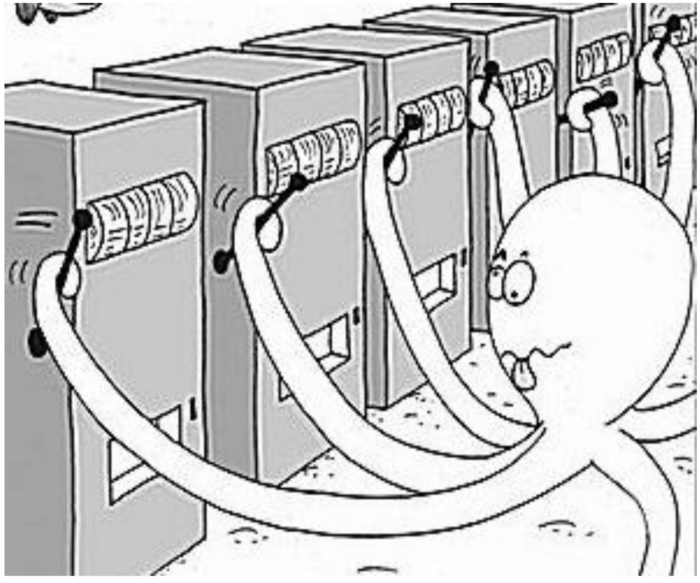
\includegraphics[scale=0.2]{./figures/MAB.png}
	\end{figure}

Bandits vs. RL (MDP)?
\end{frame}


\section{Applications}
\frame{\sectionpage}
\begin{frame}{Applications}
	\begin{itemize}
		\item \textbf{Email Campaign Problem}: Convert a potential buyer to actual buyer. Maximize user interaction with our site.
		
		\item Parameters:
		\begin{itemize}
			\item Length of the subject
			\item Time of the day the email was sent
			\item Template
			\item With links or without links ...
		\end{itemize}
		\pause
		\item Exploration vs. Exploitation!
		\pause
		\item The number of possible actions in huge. Thus we need to consider the relations between these actions and the cannot be treated separately.
		\item \textbf{Causal Model}?
	\end{itemize}
\end{frame}


\section{Causal Bandits}
\frame{\sectionpage}
\begin{frame}{Causal Bandits: Problem Setup}
\begin{itemize}
	\item We are given a causal model $\mathcal{C}$ and graph $\mathcal{G}$.
	\item All variables $\mathcal{X} = \{X_1, \dots, X_N\}$ are observable.
	\item There is a reward variable $Y$.
	\item Each variable has a discrete alphabet of size $k$.
		\item Denote $\mathrm{PA}_Y$ at round $t$ as $\bZ_{(t)} = (z_1(t), x_2(t), \dots, z_n(t))^\top$.
	\item There are $k^n$ assignments for $\bZ$, denoted as $\bZ^1, \dots, \bZ^{k^n}$.
	
\end{itemize}
\end{frame}


\begin{frame}{Causal Bandits: Problem Setup}
\begin{itemize}
	\item The learner is given the graph, $\mathcal{G}$, a set of possible interventions $\mathcal{A}$, and all inteventional distributions $P(\mathrm{PA}_Y|a)$ for $a \in \mathcal{A}$.
	\item It is assumed that $\mathcal{A}$ only consists of single node  or zero-node interventions.
	\pause
	\item Expected reward of each action $a$ and the optimal action $a^*$:
	\begin{align*}
		\mu_a &= \E[Y|a] \in [0,1]\\
		a^* &= \arg\max_{a\in\mathcal{A}} \mu_a
	\end{align*}
\end{itemize}
\end{frame}

\begin{frame}{Causal Bandits: The Sequential Game}
	\begin{itemize}
		\item In round $t$, the learner chooses the action $a_t$ based on the observation of $Y_{1}, \dots, Y_{t}$ and $\bZ_{1}, \dots, \bZ_{t-1}$ in previous rounds.
		\pause
		\item \textbf{Goal:} Maximize cumulative regret:
		\begin{equation*}
		\E[R_T] = T\mu^* - \sum_{t = 1}^{T} \E[\mu_{a_t}]
		\end{equation*}
	\end{itemize}
\end{frame}


\section{Causal Bandit Algorithms}
\frame{\sectionpage}
\begin{frame}
\frametitle{Simple Algorithms for Some Intuition}

In most bandit problems, the \textbf{Explore-Then-Commit} algorithm is analyzed first:

\begin{itemize}
	\item Perform each possible intervention $L$ times. Estimate means $\hat{\mu}_a$.
	\item Sample from $\hat{a}^* = \arg\max_{a\in\mathcal{A}}\hat\mu_a$ for $T-L$ rounds.
\end{itemize}

\begin{figure}
	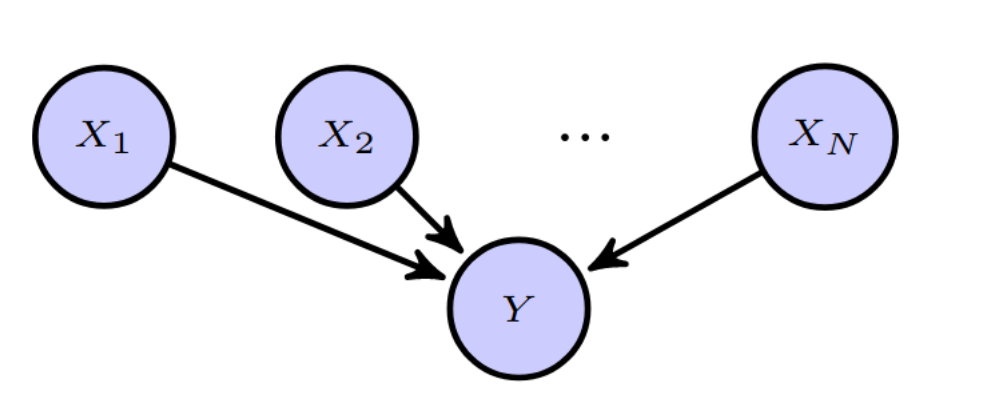
\includegraphics[scale = 0.2]{./figures/par.png}
\end{figure}


\end{frame}
%\begin{frame}
%	\frametitle{C-UCB: Causal Upper Confidence Bound}
%		\textbf{Idea 1}: Using Eq (6.7) from Elements of CI, we have:
%		
%		\begin{equation}
%			\mu_a = \sum_{j = 1}^{k^n} \E\Big[Y\big|PA_Y = \bZ^{(j)}\Big]P\Big(PA_Y = \bZ^{(j)}\big|a\Big)
%		\end{equation}
%		\pause
%		\textbf{Idea 2}: Confidence Bound!
%\end{frame}
%\begin{frame}
%\frametitle{C-UCB: Causal Upper Confidence Bound}
%
%\begin{figure}
%	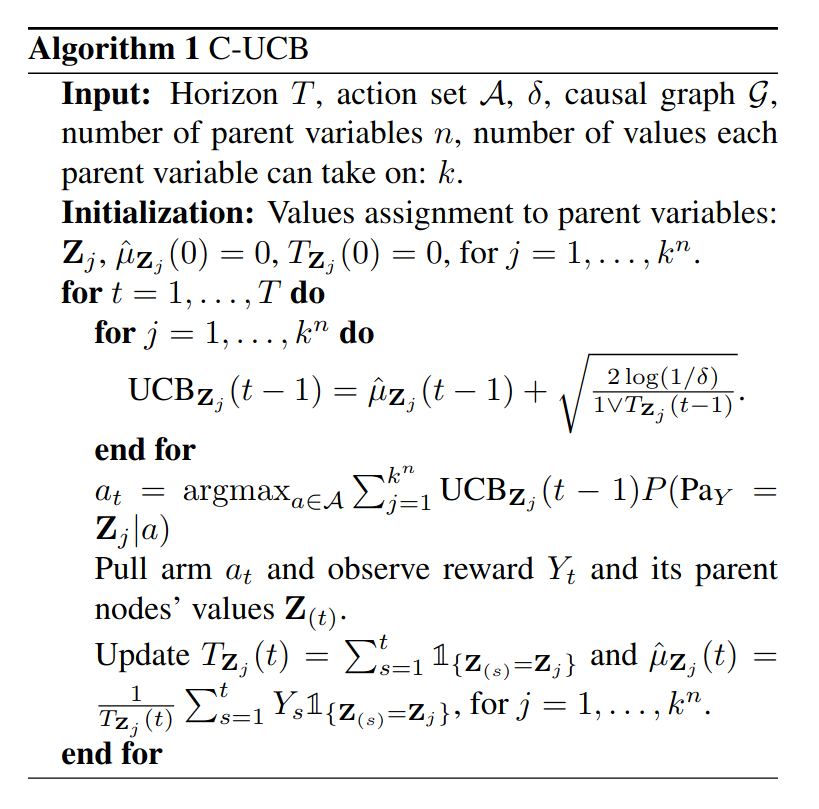
\includegraphics[scale=0.25]{./figures/C-UCB.png}
%\end{figure}
%\end{frame}


\begin{frame}
\frametitle{Causal Upper Confidence Bound}
\begin{itemize}
\item[]  For $t=1,\ldots,T$:
\vspace{0.2cm}

		\begin{enumerate}
			\item $\forall j=1,\ldots,k^n$: 
			$$\text{UCB}_{\mathbf{Z}_j}(t-1) = \hat{\mu}_{\mathbf{Z}^j}(t-1)+\sqrt{\frac{2\log(1/\delta)}{1\vee T_{\mathbf{Z}^j}(t-1)}}$$
			\item $a_t = \arg\max_{a\in\mathcal{A}} \sum_{j=1}^{k^n}\text{UCB}_{\mathbf{Z}^j}(t-1)P(\text{Pa}_Y=\mathbf{Z}^j|a)$	
			\vspace{0.2cm}
			\item Pull arm $a_t$ and observe reward $Y_t$ and its parent nodes' values $\mathbf{Z}_{(t)}$.
			\vspace{0.2cm}
			\item $\forall j=1,\ldots,k^n, $ update 
			\begin{align*}
				T_{\mathbf{Z}^j}(t) &= \sum_{s=1}^{t} \mathbf{1}_{\{\mathbf{Z}_{s}=\mathbf{Z}^j\}}\\
				\hat{\mu}_{\mathbf{Z}^j}(t) &= \frac{1}{T_{\mathbf{Z}^j}(t)}\sum_{s=1}^{t}Y_s\mathbf{1}_{\{\mathbf{Z}_{s}=\mathbf{Z}^j\}}
			\end{align*}			
		\end{enumerate}
\end{itemize}
\end{frame}


\begin{frame}
	\frametitle{C-UCB Regret Bound}
	
	\begin{theorem}
		Let $Y|_{PA_Y = \bZ^{(j)}} = \E[Y|PA_Y = \bZ^{(j)}] + \epsilon$, where $\epsilon$ is a mean zero 1-subgaussian random variable. If $\delta = 1/T^2$, the regret of C-UCB is bounded as follows:
		\begin{equation}
			\E[R_T] = \tilde{O}\Big(\sqrt{k^n T}\Big)
		\end{equation}	
	\end{theorem}
	
	We will prove this in the end (if we have time).
\end{frame}

\begin{frame}{Causal and Non-Causal Bandits}
	\begin{itemize}
		\item \textbf{Discarding causal information}: 
		
		There are $(k+1)^N$ interventions. From well known Bandit theory, $R_T = \Omega \Big(\sqrt{(k+1)^N T}\Big)$. UCB and Thompson sampling achieve this.
		
		\item \textbf{This Paper}: $R_T = O \Big(\sqrt{(k+1)^n T}\Big)$ 
		
		
		\begin{itemize}
			\item Algorithm: a variant of UCB and Thompson Sampling
			\item Assumes that we have access to $P(PA_Y|a)$ for all $a \in \mathcal{A}$.
			\item Lower bounds are not provided.
		\end{itemize}

	\end{itemize}
\end{frame}


\begin{frame}
\frametitle{Thompson Sampling}
	
	\begin{itemize}
		\item[] For $t = 1,\ldots,T$ 
					\vspace{0.2cm}
		\begin{itemize}
			\item Sample $\hat{\theta}_j(t)$ $\sim$ $N(\hat{\mu}_{\mathbf{Z}_j},\frac{1}{k_{\mathbf{Z}_j}+1})$ ,for $j = 1,\ldots,k^n$.
			\vspace{0.2cm}
			\item $\forall a\in\mathcal{A}:\;\;\hat{\mu}_a = \sum_{j=1}^{k^n}\hat{\theta}_j(t)P(\text{Pa}_Y=\mathbf{Z}_j|a)$
						\vspace{0.2cm}
			\item $a_t = \arg\max_a \hat{\mu}_a$	
						\vspace{0.2cm}
			\item Pull arm $a_t$ and observe the parent nodes values of Y denoted by
			 $\mathbf{Z}_{(t)}$ and reward $Y_t$. 
			 			\vspace{0.2cm}
			\item Update $k_{\mathbf{Z}_t}: = k_{\mathbf{Z}_t}+1$
						\vspace{0.2cm}
			\item Update $\hat{\mu}_{\mathbf{Z}_t}: = \frac{\hat{\mu}_{\mathbf{Z}_t}k_{\mathbf{Z}_t}+Y_t}{k_{\mathbf{Z}_t}+1}$
		\end{itemize}
	\end{itemize}	
\end{frame}


\begin{frame}
\frametitle{Causal Linear Bandits}
	\begin{itemize}
		\item Assume that $Y|_{\bZ} = f(\bZ)^\top \theta + \epsilon$.
		
		\item \textbf{Idea}: Regression + Confidence bound for regression + UCB algorithm.
		
		\pause
		
		\begin{theorem}
			If $||\theta||_2\leq 1$, $||f(\bZ)||_2\leq 1$, $\theta \in \mathbb{R}^d$:
			
			\begin{equation*}
			R_T = \tilde{O}(d\sqrt{T})
			\end{equation*}
			
		\end{theorem}
	\end{itemize}
\end{frame}



\section{Experiments}
\frame{\sectionpage}
\begin{frame}
\frametitle{Pure Simulation}
	\begin{columns}
		\begin{column}{0.5\textwidth}
				\begin{itemize}
				\item	Fixed conditional probabilities.
				\item 	Linear relation between $W_i$s and $Y$.
			\end{itemize}
		\vspace{-0.6cm}
		
				\begin{figure}
				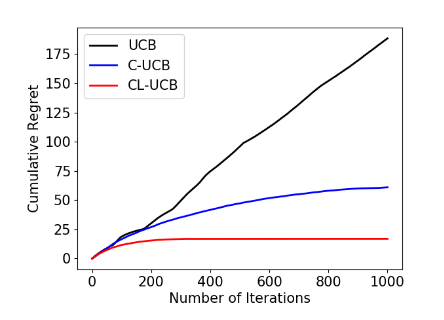
\includegraphics[scale=0.4]{./figures/plot.png}
			\end{figure}
		\end{column}
		\begin{column}{0.5\textwidth}  
			\begin{center}
				%%%%% this is a minipage, so \textwidth is already adjusted to the size of the column
				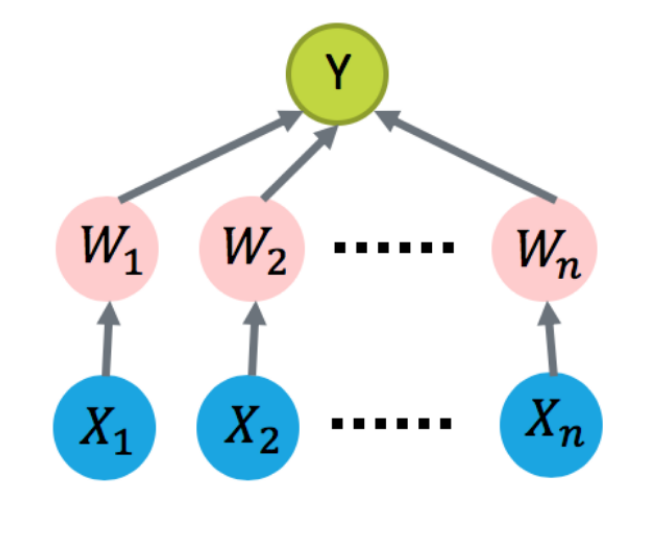
\includegraphics[scale=0.1]{./figures/graph.png}\\
				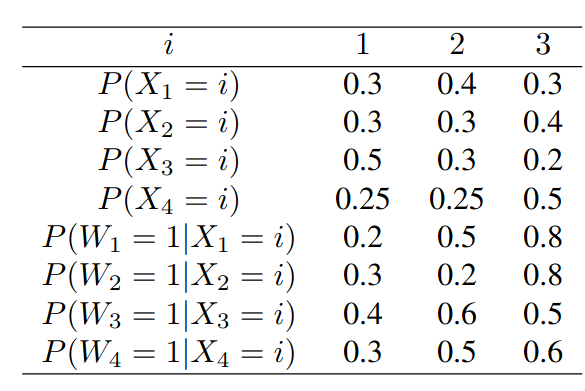
\includegraphics[width=\textwidth]{./figures/table.png}
			\end{center}
		\end{column}
	\end{columns}
\end{frame}


\begin{frame}
\frametitle{Real World Simulation!}
	\framesubtitle{EMAIL CAMPAIGN DATA}
		\begin{figure}
			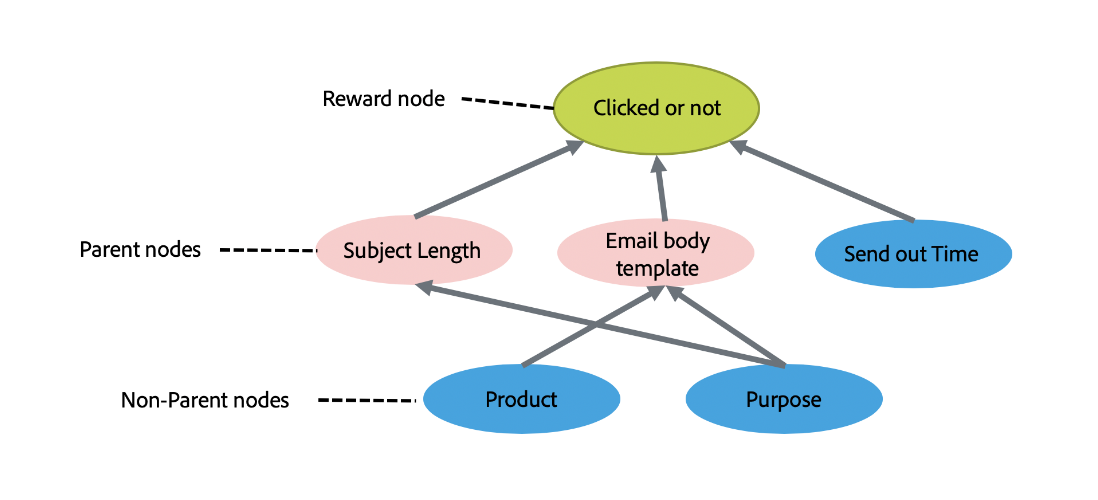
\includegraphics[scale=0.3]{./figures/exp.png}			
		\end{figure}
\end{frame}



\section{Challenges}
\frame{\sectionpage}
\begin{frame}
	\frametitle{Challenges}
	
	\begin{itemize}
		\item A much more difficult generalisation would be to consider causal bandit problems where the causal graph is completely unknown or known to be a member of class of models. 
		
		\item Work on the problem of selecting experiments to discover the correct causal graph from within a Markov equivalence class should be incorporated into a causal bandit algorithm.
		
		\item Estimating  Interventional Distributions.
	\end{itemize}
\end{frame}

\section{C-UCB Regret Bound Proof}
\frame{\sectionpage}

\begin{frame}
	\frametitle{C-UCB Regret Bound}
	Now, we will prove the C-UCB regret bound theorem.
	
	\begin{itemize}
		\item  Let $E$ be the following event:
		\begin{small}
			\begin{align*}
			\forall t\in[T], j\in [k^n], \;\; \left|\hat{\mu}_{Z^j}(t-1) - \mathbb{E}\left[Y|Pa_Y=Z^j\right]\right| \leq \sqrt{\frac{2\log(1/\delta)}{1\vee T_{Z^j}(t-1)}}.
			\end{align*}
		\end{small}
		
		\item Using union bound and subgaussanity of $\epsilon$:	$\mathbb{P}[E^c] \leq 2\delta Tk^n$.
		
		
		\pause
		\item Given that event $E$ occurs, we can write:
		
		
		
		\begin{align*}
		\text{UCB}_{\mathbf{Z}_j}(t-1) &= \hat{\mu}_{\mathbf{Z}^j}(t-1)+\sqrt{\frac{2\log(1/\delta)}{1\vee T_{\mathbf{Z}^j}(t-1)}}\geq \mathbb{E}\left[Y|Pa_Y=Z^j\right]
		\end{align*}			
	\end{itemize}
\end{frame}


\begin{frame}
	\frametitle{C-UCB Regret Bound}
	Now we can start bounding the regret:
	\begin{align*}
	R_T &= \sum_{t=1}^{T}(\mu_{a^*}-\mu_{a_t})\\&= \sum_{t=1}^{T} \left(\mu_{a^*}-\text{UCB}_{a_t}(t-1)+\text{UCB}_{a_t}(t-1)-\mu_{a_t}\right).
	\end{align*}
\end{frame}


\begin{frame}
	\frametitle{C-UCB Regret Bound}
	Hence, given that event $E$ occurs:
	
	\begin{small}
		\begin{align*}
		\mu_{a^*}-&\text{UCB}_{a_t}(t-1) \\ &=\sum_{j=1}^{k^n}\mathbb{E}\left[Y|Pa_Y=Z^j\right]P(Pa_Y=Z^j|a^*)
		-\sum_{j=1}^{k^n}\text{UCB}_{Z^j}(t-1)P(Pa_Y=Z_j|a_t)\\
		&\leq \sum_{j=1}^{k^n}\text{UCB}_{Z^j}(t-1)P(Pa_Y=Z^j|a^*)
		-\sum_{j=1}^{k^n}\text{UCB}_{Z^j}(t-1)P(Pa_Y=Z^j|a_t) \leq 0.
		\end{align*}
	\end{small}
	\pause
	The last equality follows from the way we choose $a_t$ in C-UCB: 
	$$a_t = \arg\max_{a\in\mathcal{A}} \sum_{j=1}^{k^n}\text{UCB}_{\mathbf{Z}^j}(t-1)P(\text{Pa}_Y=\mathbf{Z}^j|a)$$
\end{frame}


\begin{frame}
	\frametitle{C-UCB Regret Bound}	
	Under $E$, we have:
	{\small
	\begin{align*}
	R_T &\leq \sum_{t=1}^{T}\left(\text{UCB}_{a_t}(t-1)-\mu_{a_t}\right) \notag\\
	&=\sum_{t=1}^{T}\sum_{j=1}^{k^n}\left(\text{UCB}_{Z_j}(t-1)-\mathbb{E}\left[Y|Pa_Y=Z^j\right]\right)P(Pa_Y=Z^j|a_t) \notag\\
	&\leq \sum_{t=1}^{T} \sum_{j=1}^{k^n}\sqrt{\frac{8\log(1/\delta)}{1\vee T_{Z^j}(t-1)}}P(Pa_Y=Z^j|a_t)\notag\\
	& \leq \sum_{t=1}^{T} \sum_{j=1}^{k^n}\sqrt{\frac{8\log(1/\delta)}{1\vee T_{Z^j}(t-1)}}\left(\underbrace{P(Pa_Y=Z^j|a_t)-\mathbf{1}_{\{Z_{(t)}=Z^j\}}}+\underbrace{\mathbf{1}_{\{Z_{(t)}=Z^j\}}}\right). \label{equ:UCB_azuma}
	\end{align*}
	}
\end{frame}

\begin{frame}
	\frametitle{C-UCB Regret Bound}	
	\begin{itemize}
		\item The first part:
			\begin{align*}
			|X_t-X_{t-1}|^2 &= \left|\sum_{j=1}^{k^n}\sqrt{\frac{8\log(1/\delta)}{1\vee T_{Z^j}(t-1)}}\left(P(Pa_Y=Z^j|a_t)-\mathbf{1}_{\{Z_{(t)}=Z^j\}}\right)\right|^2\\
			&\leq 32\log(1/\delta).
			\end{align*}			
			Hence it has the bounded difference property.
					
		\item The second part:
			\begin{align*}
			\sum_{t=1}^{T} \sum_{j=1}^{k^n}\sqrt{\frac{8\log(1/\delta)}{1\vee T_{Z^j}(t-1)}}\mathbf{1}_{\{Z_{(t)}=Z^j\}} &\leq \sum_{j=1}^{k^n}\int_{0}^{T_{Z^j}(T)}\sqrt{\frac{8\log(1/\delta)}{s}} ds\\
			&\leq \sum_{j=1}^{k^n} \sqrt{32T_{Z^j}(T)\log(1/\delta)}\\
			&\leq \sqrt{32k^nT\log(1/\delta)}.
			\end{align*}			
	\end{itemize}
\end{frame}


\begin{frame}
	\frametitle{C-UCB Regret Bound}
	Azuma-Hoeffding: \begin{align*}
	P(|X_T|>\sqrt{k^nT\log(T)}\log(T)) \leq \exp\left(-\frac{k^n\log^3(T)}{32\log(1/\delta)}\right).
	\end{align*}
	
	Take $\delta = 1/T^2$. With probability $$1-P(E^c)-\exp\left(-\frac{k^n\log^2(T)}{64}\right) = 1-2k^n/T-\exp\left(-\frac{k^n\log^2(T)}{64}\right),$$ the regret can be bounded by
	\begin{align*}
	R_T \leq 16\sqrt{k^nT\log(T)}\log(T).
	\end{align*}
	Thus the expected regret can be bounded by:
	\begin{align*}
	\mathbb{E}\left[R_T\right] &\leq P(E^c)\times 2T+\exp\left(-\frac{k^n\log^2(T)}{64}\right)\times 2T+\sqrt{64k^nT\log(T)}\log(T)\\
	&\leq C\sqrt{k^nT\log(T)}\log(T).
	\end{align*}
\end{frame}




\end{document}
